\section{Introduction}
% no \IEEEPARstart

\subsection{History}
Blockchain was introduced for the first time in 2008, when Satoshi
Nakamoto, an anonymous Japanese\footnote{Actually, experts think that Satoshi
Nakamoto is an alias for a group of people and that no one with that name
really exists.} user designed it in order to create a virtual currency,
Bitcoin. Since then, the Blockchain technology has developed to new frontiers,
establishing new ways to think money and payments. Furthermore, it is currently
studied in different fields than the financial one.

\subsection{Paper structure}

This paper is organized as follows: Section~\ref{sec:block_design} describes
how Blockchain is designed and how it works, making a technical analysis of this
technology and talking about its security and privacy issues, while
Section~\ref{sec:crypto_corr} provides an overview of the
use of this application in its main field: cryptocurrency.
Section~\ref{sec:beyond_crypto} describes new ways to use this technology and
the possible threats, while Section~\ref{sec:smart_contracts} will briefly talk
about smart contracts, with its pros and cons about security and privacy.

\section{Blockchain design}
\label{sec:block_design}
Blockchain was designed in order to solve the double-spending problem in
online transactions, where a single digital token is used to pay more than one
time, without any third party checking\cite{nakamoto08}. To achieve this, it
relies on a peer-to-peer system, where every user hold a copy of the whole
transaction history.

Every transaction is hashed and stored in a block, and blocks are connected in
a list. These are generated by members in the network, with a process called
``mining''. When users are mining, they contribute generating and validating
new blocks. When a block is generated, a reward is released from the network,
compensating the users that spent computational time to generate and validate
the block.

Blockchain implementations, especially for the financial applications, do not
allow to modify or to delete saved data, but only to add new information. This
prevents any transaction forgery by attackers, although it does not stop the
possibility for an attacker to add new material that invalidates the old one.

\subsection{Technical Analysis}

As mentioned above, Blockchain is composed of three different
parts\cite{sok15}: transactions, blocks concatenated to form a graph and a
peer-to-peer network. In this section we will see every component and how it 
behaves.

\subsubsection{Transaction}
It represents a value's movement between user $A$ and another (let's
say $B$). A transaction contains an array of outputs and an array of
inputs\cite{sok15}: the sum of outputs must be less or equal than the sum of
the inputs.
This container is usually hashed with SHA-256, in order to have a
unique ID.

A transaction changes the blockchain state, making it a list of growing
transactions.
In order to validate a transaction, we need to sign it in some way. Asymmetric
keys are mandatory in this process.

If $A$ wants to send money to $B$ it needs to:
\begin{enumerate*}[label=\roman*)]
 \item sign (with her private key) the previous hashed transaction and sign the
public key of the next owner ($B$);
 \item save all the signatures in the chain.
\end{enumerate*}

\begin{figure}[ht]
 \centering
 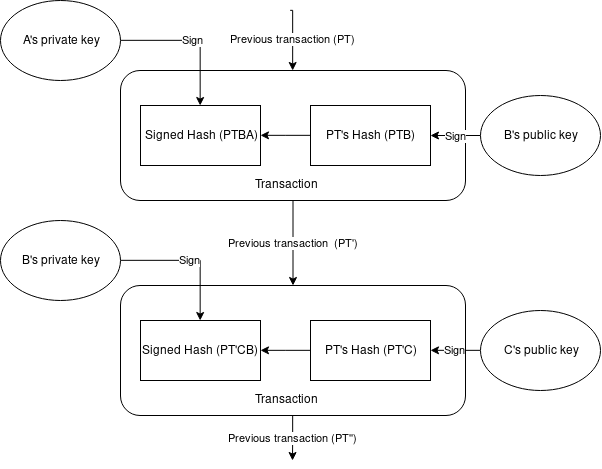
\includegraphics[scale=0.42]{transaction}
 \caption{A typical series of transactions}
\end{figure}

Several problems arise from this:
\begin{enumerate*}[label=\roman*)]
 \item apparently no one can guarantee the transaction validity;
 \item $A$ could spend two times the same value.
\end{enumerate*}

\paragraph*{Transaction Validity}
The list of transactions can be verified thanks to the chain of ownership:
in fact, every user has a local copy of the whole transaction history so it has
the possibility to check it and define if the transaction is valid.
This possibility enable nodes to check autonomously the transaction validity,
thus allowing them to reject the malformed or forged one without needing any
third-party~\cite{nakamoto08}.

\paragraph*{Double spending problem}
The easiest solution could be ensuring a third-party to check all the
transactions, searching for possible frauds. This would imply to establish an
entity that acts like a bank, against the Blockchain design. On top of this,
the entity could act arbitrarily, for instance denying payments to specific
groups of people.

To ensure that $A$ is giving money that were not already used, $B$ needs to
check the transactions. In these case, only the earliest is
valid\cite{nakamoto08}. This leads to two minor problems:
\begin{enumerate*}[label=\roman*)]
 \item $B$ needs to have a list of all the transactions;
 \item $A$ could try to pay $B$ and $C$ with the same amount of money in a very
short span of time, causing dispute to who should receive the payment.
\end{enumerate*}

\paragraph*{Transactions updates}
\label{TU}
$B$ needs all the transactions in order to be able to recognize a possible
fraud from $A$. To accomplish this all the transactions have to be broadcast to
everyone in the network, making it publicly available.

\paragraph*{Timestamps}
To solve this problem every transaction need to be timestamped. A timestamp is
given to a transaction and it is added to its hash. In order to eliminate every
possibility of alterations, the previous transaction timestamp is added into
the hash too\cite{nakamoto08}.

\subsubsection{Block}
A set of transactions is put in a set together called \textit{block}. Every
block has a link to the previous one and another to the next one, forming
indeed a \textbf{blockchain}.

\label{sub:fork}
Sometimes it could happen that a list of blocks forks from the main chain. In
this cases, the shortest chain will be eventually discarded, and all the miners
will restart working on the longest one\cite{sok15}. The forking process can be
a vector for attacks, and we will talk about it in~\ref{sub:tfp}.

\subsubsection{Peer-to-Peer Network}

Blockchain is a sort of peer-to-peer database, meaning that there is not a
central server that store all the data, but the information is spread through
all the peers.
In this way anyone in the network owns a copy of the whole transaction history.
The first time a peer connects to the network it has to wait and get in sync
with the other peers. In the meantime, no operation is permitted. A Blockchain
size can grow a lot over the years. For example, Bitcoin's
blockchain\footnote{N.B.: this is an 8 years old database.} size is roughly
100GB\footnote{GB = GigaByte}. This could be an issue especially for the new
members of the network.
This great amount of data can be reduced, though, if transactions are hashed in
a Merkle tree, a data structure similar to a binary tree. In a complete binary
tree we have that every internal node has two children. A Merkle tree is
a complete binary tree where every internal node has a label that is the hash
of the labels or values of its children\cite{szydlo04}. The advantage of using
this technique is that only the root of the tree needs to be stored in the
block and not all the transactions\cite{nakamoto08} (thus saving space), on the
other hand this require additional computational time to check all the
transactions in the tree. Moreover, there is the possibility of what is called a
\textit{second preimage} attack on the Merkle root, where an attacker could
change part of the tree with another that has the same hash\cite{rogaway04}. In
order to mitigate this attack a preimage attack resistant hash algorithm should
be chosen.


As said in \ref{TU}, every transaction is broadcast through the network so when
the miners mine a new block every peer starts to download it.

\subsection{Mining algorithms}
In a Blockchain, peers can emit new transactions in the network. These
need to be added into blocks and these blocks need to be concatenated in order
to form a blockchain. This process is performed by \textbf{miners}.
There are different ways to attach blocks, and this depends on the mining
algorithm used: first of all, a miner could be randomly elected to mine the
next block. This approach works only if all the miners are trusted, because if
there is at least one miner that is infected or not trusted he could mine a
block with non-authorized transaction, thus attacking the blockchain. Another
solution could be allowing only a very-restricted number of computers to mine
the blockchain: supposing they are all trustworthy this approach would fail the
initial Blockchain design, centralizing the network.
A solution that has kicked off well seems to be the one where all the nodes in
the network are allowed to mine, and the first one who solves a
computational-intensive puzzle can attach the block to the existing chain,
receiving a reward for the work it made. We will see an example of this
approach, called \textbf{proof-of-work}.


\paragraph{Proof-of-Work}

With this method, peers usually have to solve a computational 
intensive problem, based on the \textit{one-way} hash property. It says that 
given an hash $h$ it is computationally infeasible to find $x$ such that $H(x) 
= h$.
In every block a \textit{nonce} field is added, and miners have to found an
hash for that block that its value is less than the previous one\cite{sok15}.
The only solution to solve is to try every possible nonce combination that
result in an hash that is less than the previous one. Every time a new block is
added to the blockchain, the problem becomes computationally more difficult to
solve.
When two different miners found a different solution a fork can happen. As
already said above (\ref{sub:fork}), only the longest chain is kept eventually.

Every time a puzzle is solved the miners (that can form groups called
\textit{pools}) typically gain a reward. This reward is important to keep miners
working and processing transactions.

This method was proposed for preventing abuse such e-mail spam, and for this
reason it is called \textit{proof-of-work}~\cite{back02}, but it is not the 
only one existing, and different \textit{proof-of-work} algorithms might have 
different problems to solve.

\subsection{The forking problem}
\label{sub:tfp}

The last block in a blockchain is defined as \textit{head}. When a
\textbf{fork} happen, new heads are formed.

After a miner finishes its proof-of-work solving the computational puzzle
it will try to attach its block to the chain, in order to gain a reward (if
any). There is the possibility that two miners will find a good solution for
the same block and that they will try to attach to the blockchain at the same
time: this will result in the blockchain splitting, operation also known as
\textbf{forking}. In this kind of forks miners will work on one branch of the
chain, attaching blocks: eventually, one of them will prevail on the others.
When this happens, the other branches will be discarded, and the blocks
forming those branches will become \textit{orphan blocks}~\cite{decker13}.
Miners that mine orphan blocks will likely not receive any reward.

Usually this kind of forks are not a threat when the computational power is
distributed in an uniform manner through the network, but when one member has a
lot of it it could be a security issue. In fact, a member could try to carry 
out a \textit{fork attack}. In order to succeed, the attacker branch (let's call 
it $B_A$) needs to ``race''~\cite{nakamoto08} with the honest one (that for the
sake of simplicity we call it $B_H$) and to overtake it. To be able to have
$B_A > B_H$ the attacker needs to have more computational power than the rest of
the network, in other words more than $50\%$ of it.
If this attack succeed, the attacker is able to make her chain ($B_A$) with
altered transaction the honest chain ($B_H$).
In a financial application, the attacker will not be able to add unlimited
founds to her wallet or to change arbitrary data (since every transactions are
signed and honest nodes will not accept forged one), but she will be able to
change her own money movements and to take them back.

Forks are used in different ways to handle mining software updates easily, or
even to change on purpose the content of a transaction\cite{sok15}. In the
first case these kind of forks are called \textit{soft forks} where there is a
change in the Blockchain structure that is retro-compatible with the current
chain rules, in the second case these forks are defined as \textit{hard forks}
and the changes are so deep that miners that have not updated their mining
software will see new transactions as invalid. An example of hard forks is what
split the cryptocurrency Ethereum in two versions, Ethereum Classic and
Ethereum.
